\documentclass[10pt]{standalone}
\usepackage[utf8]{inputenc}
\usepackage{pgf,tikz,pgfplots}
\pgfplotsset{compat=1.15}
\usepackage{mathrsfs}
\usetikzlibrary{arrows,patterns}
\pagestyle{empty}
\begin{document}

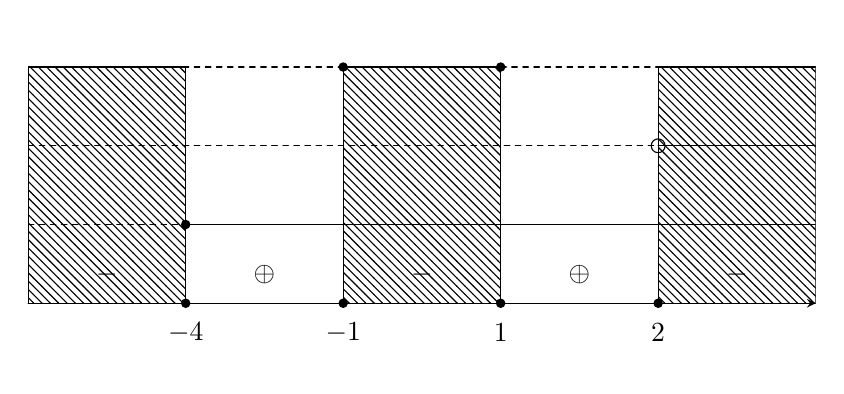
\begin{tikzpicture}[line cap=round,line join=round,>=triangle 45,x=1.0cm,y=1.0cm]
\begin{axis}[
x=1.0cm,y=1.0cm,
axis x line=middle,
axis y line=none,
ticks=none,
xmin=0.0,
xmax=10.0,
ymin=-0.8,
ymax=3.5,
xtick={-0.0,1.0,...,10.0},
ytick={-0.0,1.0,...,3.0},]
\draw[pattern=north west lines] (0,0) rectangle (2,3.0);
\draw[pattern=north west lines] (4,0) rectangle (6,3.0);
\draw[pattern=north west lines] (8,0) rectangle (10,3.0);
\clip(-0.5,-1.0) rectangle (10.5,3.5);
\draw  (2.,1.)-- (2.,0.);
\draw  (4.,3.)-- (4.,0.);
\draw  (6.,3.)-- (6.,0.);
\draw  (8.,2.)-- (8.,0.);
\draw [dash pattern=on 2pt off 2pt] (0.,1.)-- (2.,1.);
\draw  (2.,1.)-- (10.,1.);
\draw [dash pattern=on 2pt off 2pt] (0.,2.)-- (8.,2.);
\draw  (8.,2.)-- (10.,2.);
\draw [dash pattern=on 2pt off 2pt] (0.,3.)-- (4.,3.);
\draw  (4.,3.)-- (6.,3.);
\draw [dash pattern=on 2pt off 2pt] (6.,3.)-- (10.,3.);
\begin{scriptsize}
\draw [fill=black] (2.,0.) circle (1.5pt);
\draw (2.0,-0.37) node {$-4$};
\draw [fill=black] (4.,0.) circle (1.5pt);
\draw (4.0,-0.37) node {$-1$};
\draw [fill=black] (6.,0.) circle (1.5pt);
\draw (6.0,-0.37) node {$1$};
\draw [fill=black] (8.,0.) circle (1.5pt);
\draw (8.0,-0.37) node {$2$};
\draw [fill=black] (2.,1.) circle (1.5pt);
\draw (8.,2.) circle (2.5pt);
\draw [fill=black] (4.,3.) circle (1.5pt);
\draw [fill=black] (6.,3.) circle (1.5pt);
\draw (1.0,0.37) node {$-$};
\draw (3.0,0.37) node {$\oplus$};
\draw (5.0,0.37) node {$-$};
\draw (7.0,0.37) node {$\oplus$};
\draw (9.0,0.37) node {$-$};
\end{scriptsize}
\end{axis}
\end{tikzpicture}
\end{document}